\section{REAL CASE STUDY: OPTIMAL HEATER SCHEDULING} In this section we show a real application of DPC. In particular we create both an EnergyPlus and a random forest model for energy consumption, that we use to compare performance, and random forest models for power consumption and room temperatures to be used in the closed-loop simulations. These models are created using real data from the period March $11^{th}$ - May $15^{th}$ $2016$ of an off-grid house located in L'Aquila (Italy). We apply DPC to obtain an optimal scheduling policy for the heating system and compare the results with a classical ON/OFF controller. In the following we first describe the house and the models we created for the simulation, then we set up our optimization problem and show performance results.

\subsection{Description of the house} TBD

\subsection{EnergyPlus model} TBD

\subsection{Random forest models} We create $2$ different sets of models $S_1$ and $S_2$ using random forests. In each set we have a model for the power consumption of the house and $4$ models that describe the evolution of the room temperature in each of the $4$ rooms. Models in $S_1$ are used as plant simulator of the house and are created using the classical random forest algorithm, while models in $S_2$ are used for predictions in the DPC algorithm and are then created using the methodology provided in Section \ref{SS:dpcrf}. The non-manipulated features in $\tX^d$ are the disturbance data (relative humidity, atmospheric pressure, outside air temperature, sun radiation, wind, time of the day and day of the week) and the states (temperature of $4$ rooms). The manipulated feature in $\tX^c$ is the flow rate ($[m^3/h]$). All this features are used to create models in $S_1$ and the power model in $S_2$, while disturbance data, only state temperature $x_i$ and flow rate are used to identify $\hat{\Theta}^{T}_{\tT^i_j}$ for temperature models in $S_2$.

\begin{table}[h!]
	\centering
	\caption{Model accuracy of models in $S_1$.}
	\captionsetup{justification=centering}
	\begin{tabular}{c|c|c|c|c|c}
		\toprule
		$S_1$     & Power & T. room $1$ & T. room $2$ & T. room $3$ & T. room $4$  \\ 
		\midrule
			$S_1$ & $num$ & $0.627$        & $158$          & $158$           & $158$\\
			$S_2$ & $num$ & $0.673$        & $81$           & $158$           & $158$\\
		\bottomrule
	\end{tabular}
	\label{T:S1accuracy}
\end{table}

\begin{table}[h!]
	\centering
	\caption{Model accuracy of models in $S_2$.}
	\captionsetup{justification=centering}
	\begin{tabular}{c|c|c|c|c|c}
		\toprule
		$S_1$     & Power & T. room $1$ & T. room $2$ & T. room $3$ & T. room $4$  \\ 
		\midrule
		$S_1$ & $num$ & $0.627$        & $158$          & $158$           & $158$\\
		$S_2$ & $num$ & $0.673$        & $81$           & $158$           & $158$\\
		\bottomrule
	\end{tabular}
	\label{T:S2accuracy}
\end{table}


\subsection{DPC and bang-bang control problems} TBD

\paragraph{DPC}
We want to optimize the ON/OFF heater schedule in order to minimize power consumption of the house while keeping temperature of room $3$ within a comfort range. We choose to constraint only one room temperature since in the house it is not possible to control temperature in each room. This is because as explained in Section TBD, the same flow controls the temperature of all rooms simultaneously. We also allow violations $\eps^{min},\eps^{max}$  of temperature bounds to guarantee feasibility of the algorithm. We include these violations in the objective function to minimize and we compare performance considering different weights. The problem is setup as follows:
\begin{align}
	\begin{aligned}
		\min_{\tX^c,\eps_j^{min},\eps_j^{max}} & \ \ \ \sum_{j=1}^{N} Q{\tP}_{\mathrm{k+j|k}}^2 +  \lambda_{min}\parallel\eps^{min}\parallel_2 + \lambda_{max}\parallel\eps^{max}\parallel_2 \\
		\text{s.~t. }& \ \ \ \ \ {\tP}_{\mathrm{k+j|k}} =  \hat{\Theta}^{T}_{\tP_j} [ 1,\tX^c_{\mathrm{k|k}},\dots,\tX^c_{\mathrm{k+j-1|k}} ]^T \\
					 & \ \ \ \ \ \tT^1_{\mathrm{k+j|k}} =  \hat{\Theta}^{T}_{\tT^1_j} [ 1,\tX^c_{\mathrm{k|k}},\dots,\tX^c_{\mathrm{k+j-1|k}} ]^T \\
					 & \ \ \ \ \ \tT^2_{\mathrm{k+j|k}} =  \hat{\Theta}^{T}_{\tT^2_j} [ 1,\tX^c_{\mathrm{k|k}},\dots,\tX^c_{\mathrm{k+j-1|k}} ]^T \\
			 	 	 & \ \ \ \ \ \tT^3_{\mathrm{k+j|k}} =  \hat{\Theta}^{T}_{\tT^3_j} [ 1,\tX^c_{\mathrm{k|k}},\dots,\tX^c_{\mathrm{k+j-1|k}} ]^T \\
				 	 & \ \ \ \ \ \tT^4_{\mathrm{k+j|k}} =  \hat{\Theta}^{T}_{\tT^4_j} [ 1,\tX^c_{\mathrm{k|k}},\dots,\tX^c_{\mathrm{k+j-1|k}} ]^T \\					
					 & \underline{\tT}_{\mathrm{k+j-1|k}}-\eps^{min}_j \leq \tT^3_{\mathrm{k+j|k}} \leq \overline{\tT}_{\mathrm{k+j-1|k}} + \eps^{max}_j\\
					 & \ \ \ \ \ \ \ \ \tX^c_{\mathrm{k+j-1|k}} = 0 \lor \tX^c_{\mathrm{k+j-1|k}} = 0.35\\ 
					 & \ \ \ \ \ \ \ \ \ \ \ \ \ \ \ \eps_j \geq 0, \ j = 1,\dots,N.
	\end{aligned}
	\label{E:DPCrealcase}
\end{align}
\paragraph{Bang-bang controller}
This is the classical controller used to keep temperature within a range. It switch the heater on when the temperature goes under the temperature lower bound and switch it off when the temperature goes over the temperature upper bound. The advantage is that it is very simple to install but it uses more energy than what it is actually needed to achieve the task.
\subsection{Simulation Results} To avoid to many oscillations we set up both control problems such that when the heater is activated then it must stay active for at least $20$ minutes.

\begin{figure}[h!]
	\subfigure[Comparison of temperature of room $3$ obtained with DPC and bang-bang controller.]{
		\label{F:Temperatures_small}
		\centering
		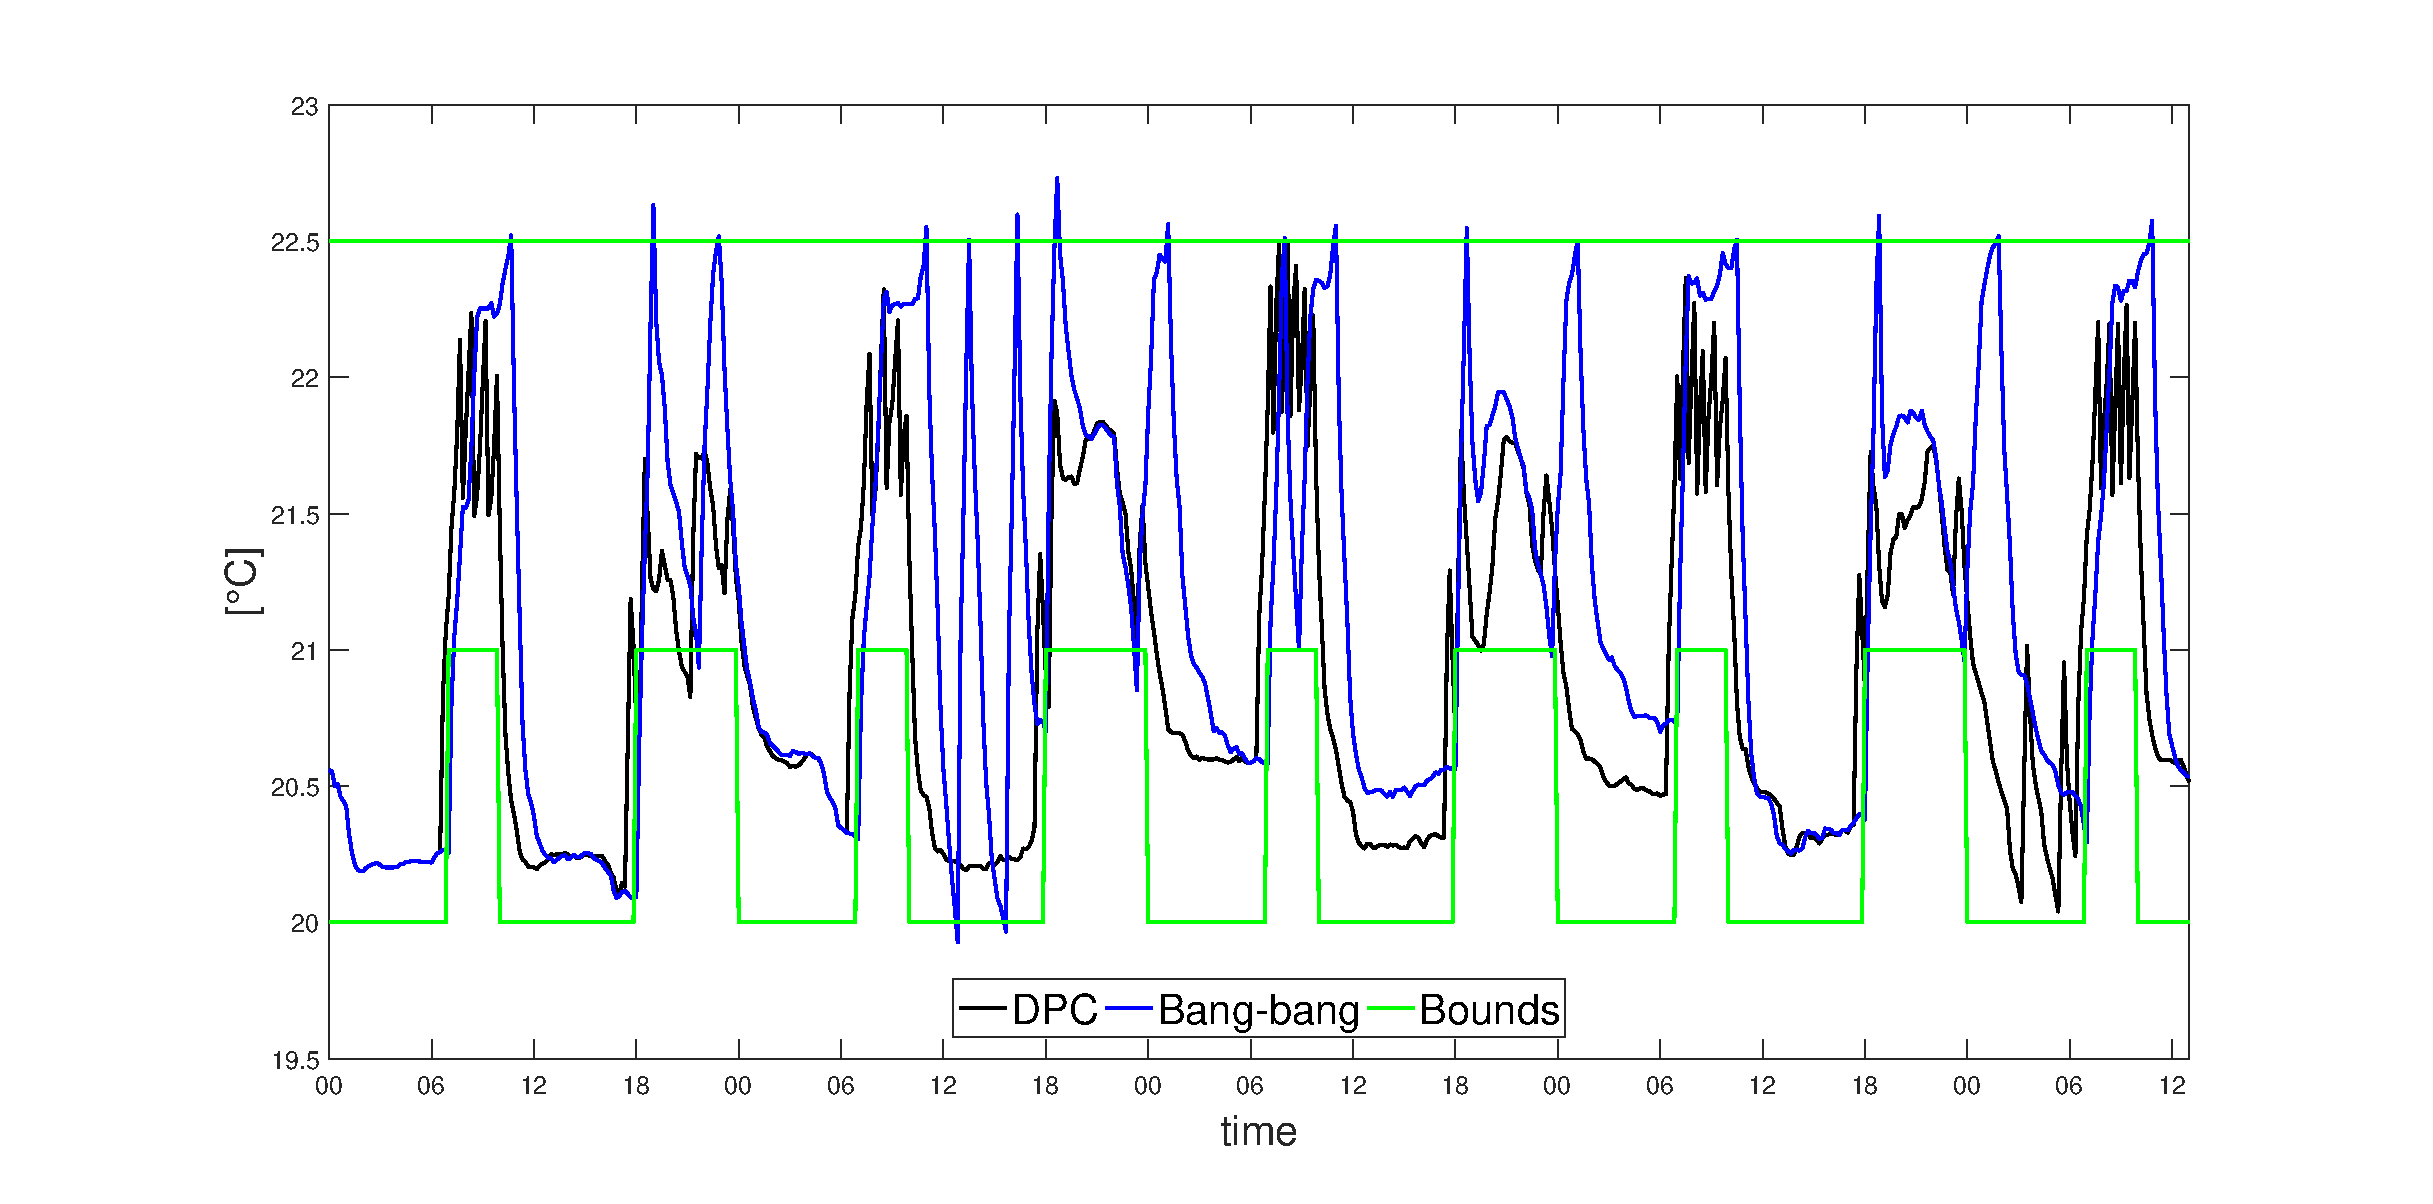
\includegraphics[width=22pc]{figures/Temperatures_small.eps}
	}
	\subfigure[Input schedules obtained from DPC and bang-bang controller.]{
		\label{F:Inputs_small}
		\centering
		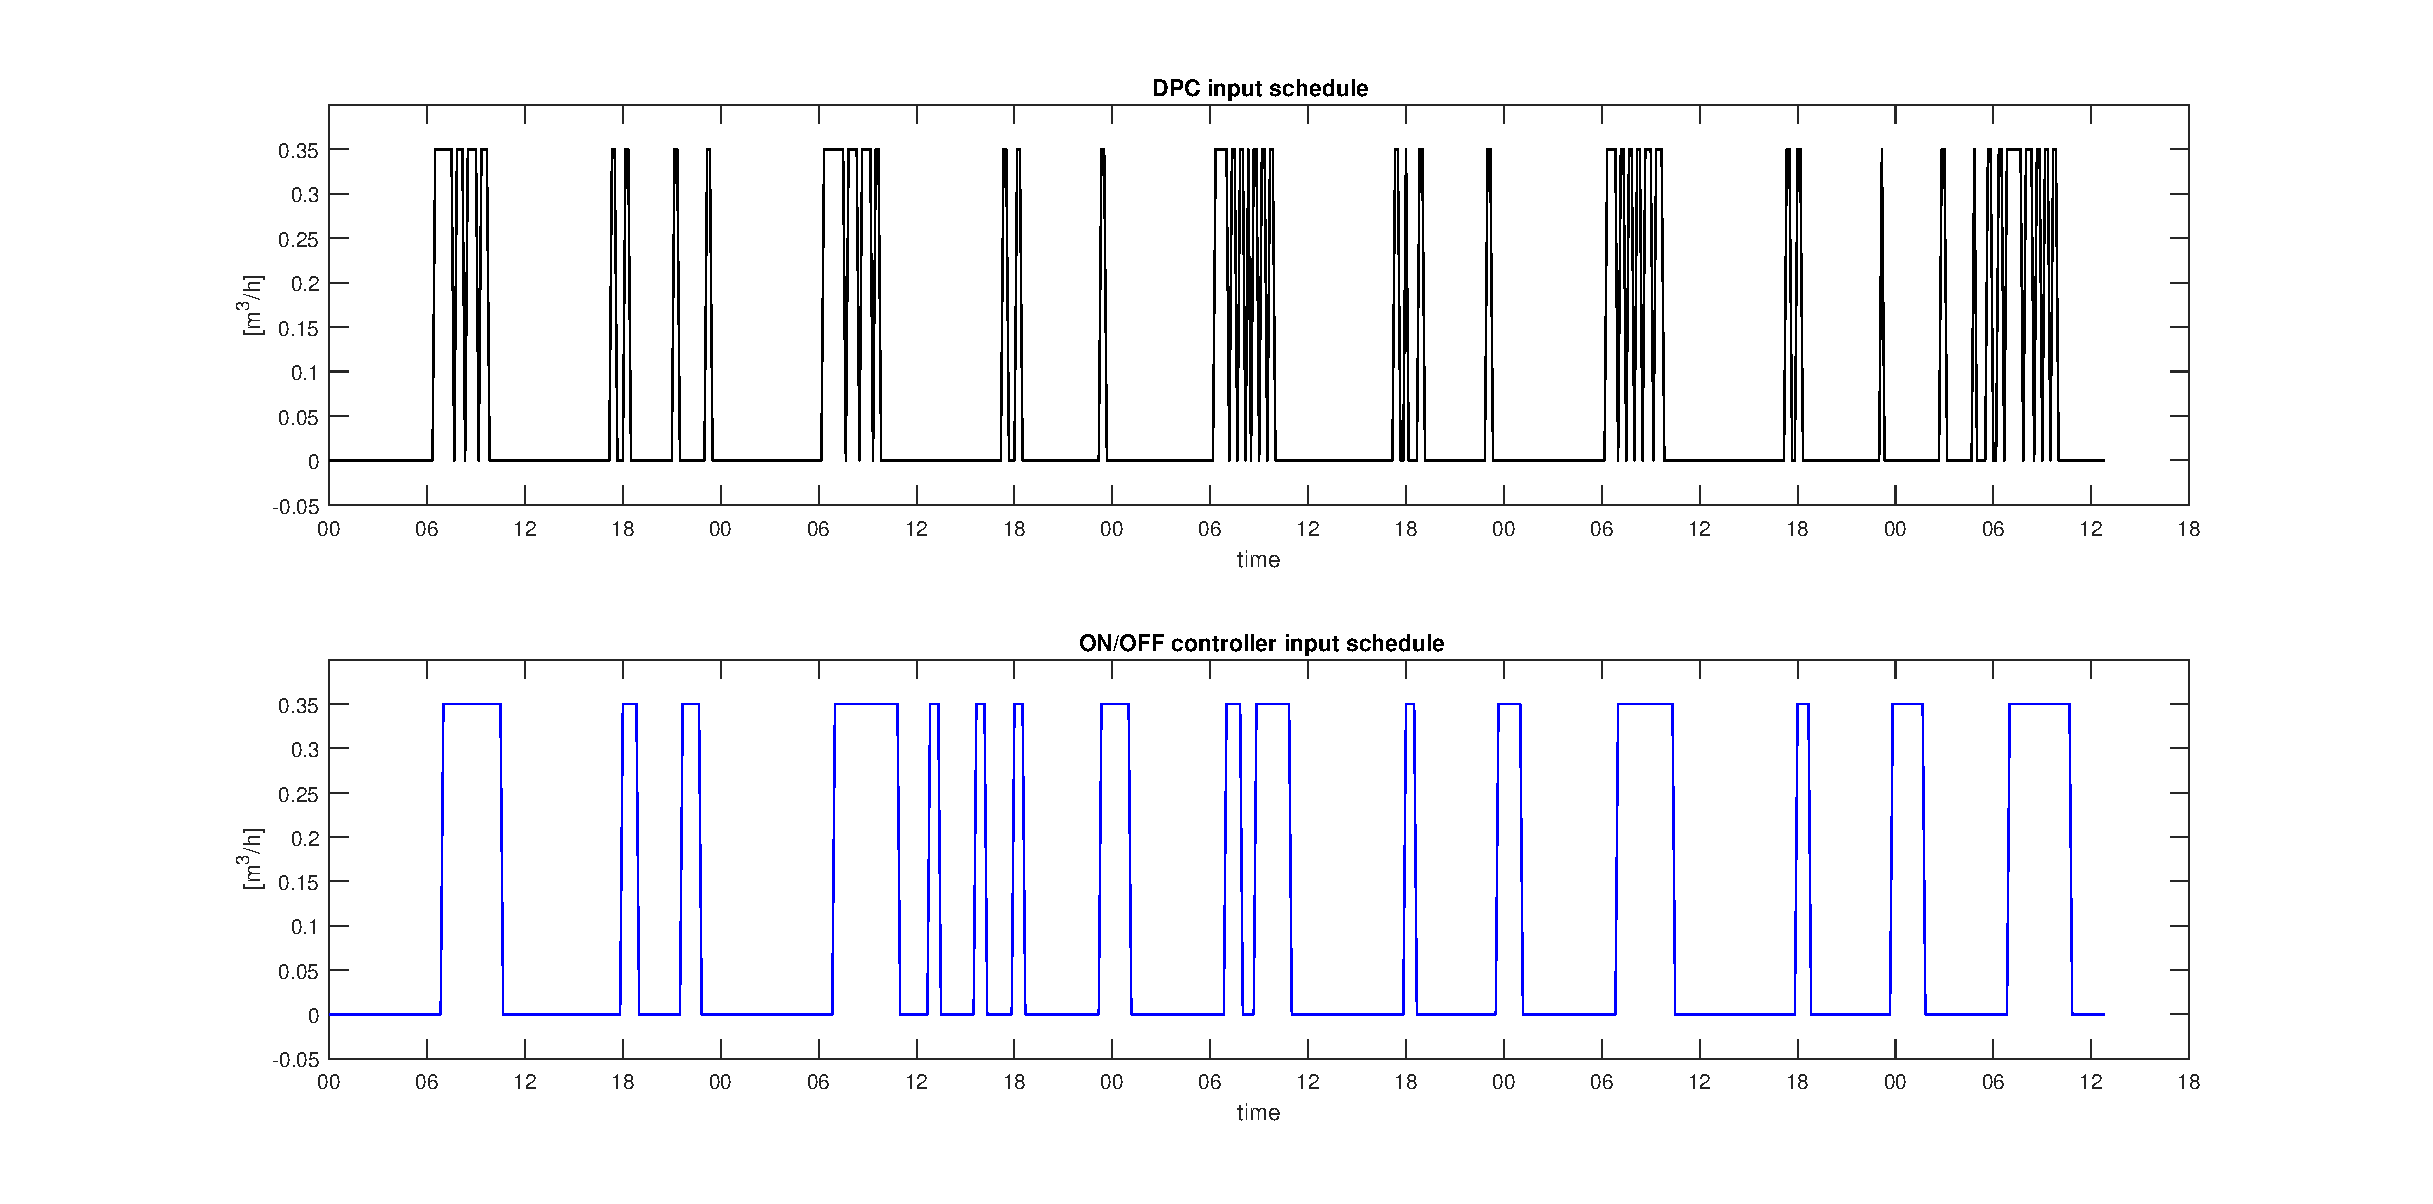
\includegraphics[width=22pc]{figures/Inputs_small.eps}
	}
	\caption{Comparison of DPC and bang-bang control performance.}
	\captionsetup{justification=centering}
	\label{F:Comparison_small}
\end{figure}

\begin{figure}[h!]
	\subfigure[Comparison of temperature of room $3$ obtained with DPC and bang-bang controller.]{
		\label{F:Temperatures_all}
		\centering
		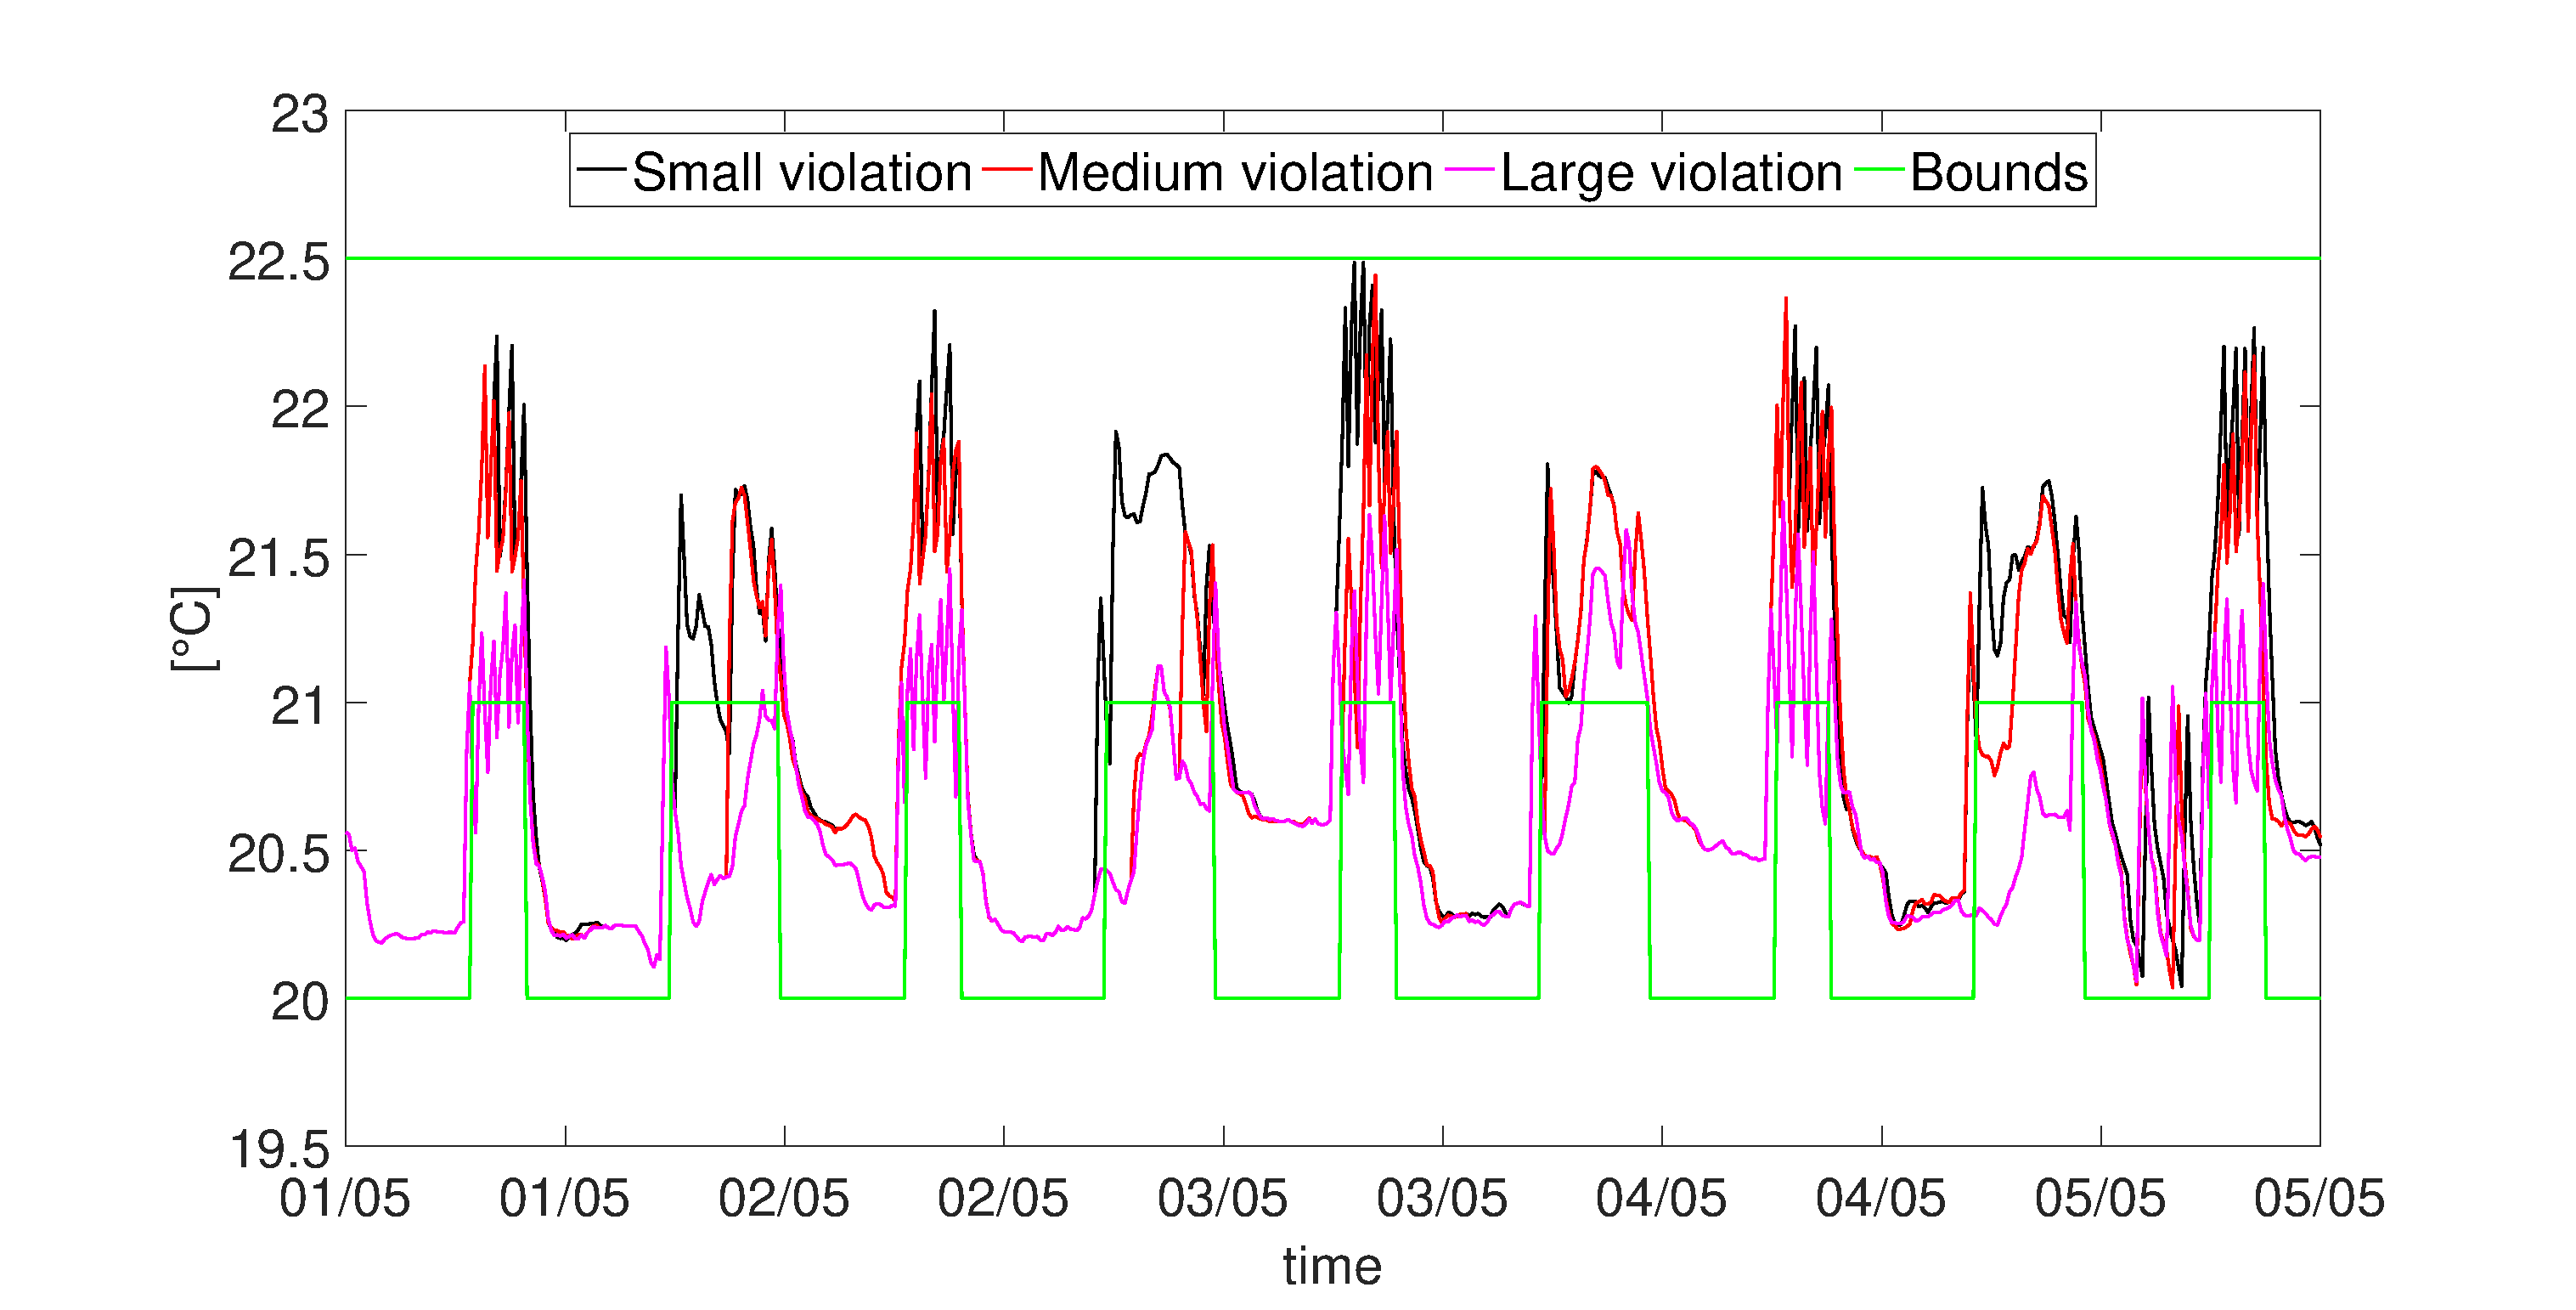
\includegraphics[width=22pc]{figures/Temperatures_all.eps}
	}
	\subfigure[Input schedules obtained from DPC and bang-bang controller.]{
		\label{F:Energy_all}
		\centering
		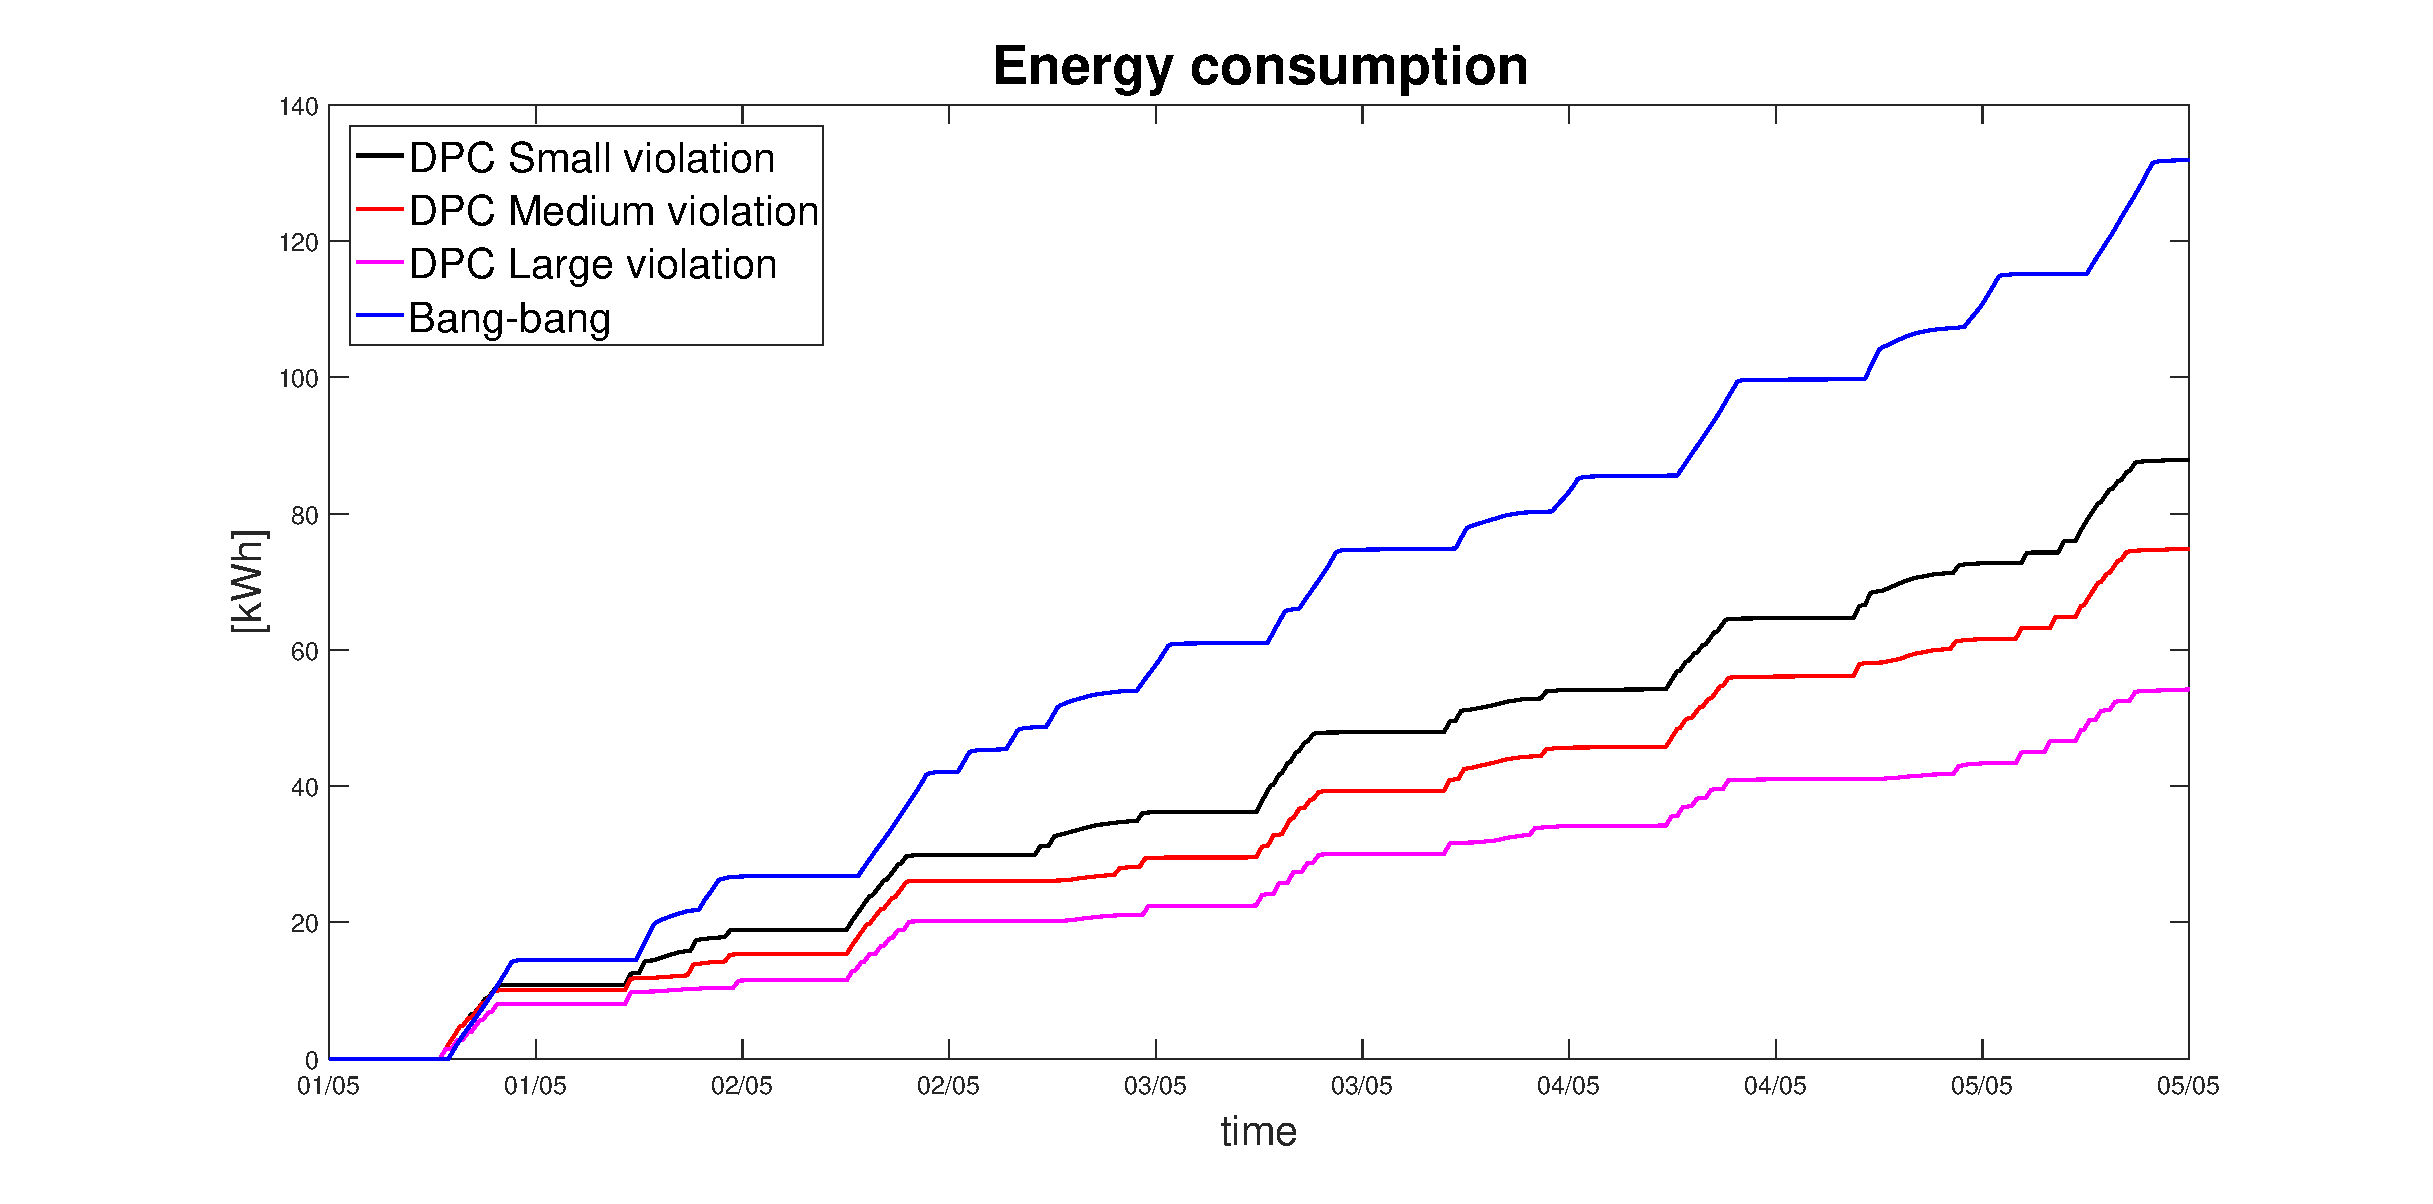
\includegraphics[width=22pc]{figures/Energy_all.eps}
	}
	\caption{Comparison of DPC and bang-bang control performance with different violations.}
	\captionsetup{justification=centering}
	\label{F:Comparison_small}
\end{figure}

\paragraph{Energy-efficiency improvements}